\chapter{Sets of reference organisms}
\label{appendixdorota}
The next pages contain the list of organisms in the subsets created by two different taxonomic criteria: ``nearest'' - going from the reference organism to the root taking all the organisms in the resulting taxa - and ``level'' - the tree is successively cut and one organism is taken from each one of the resulting groups. A representation of whole taxonomic tree (black) with the selected organisms (red) is also included in the next pages.

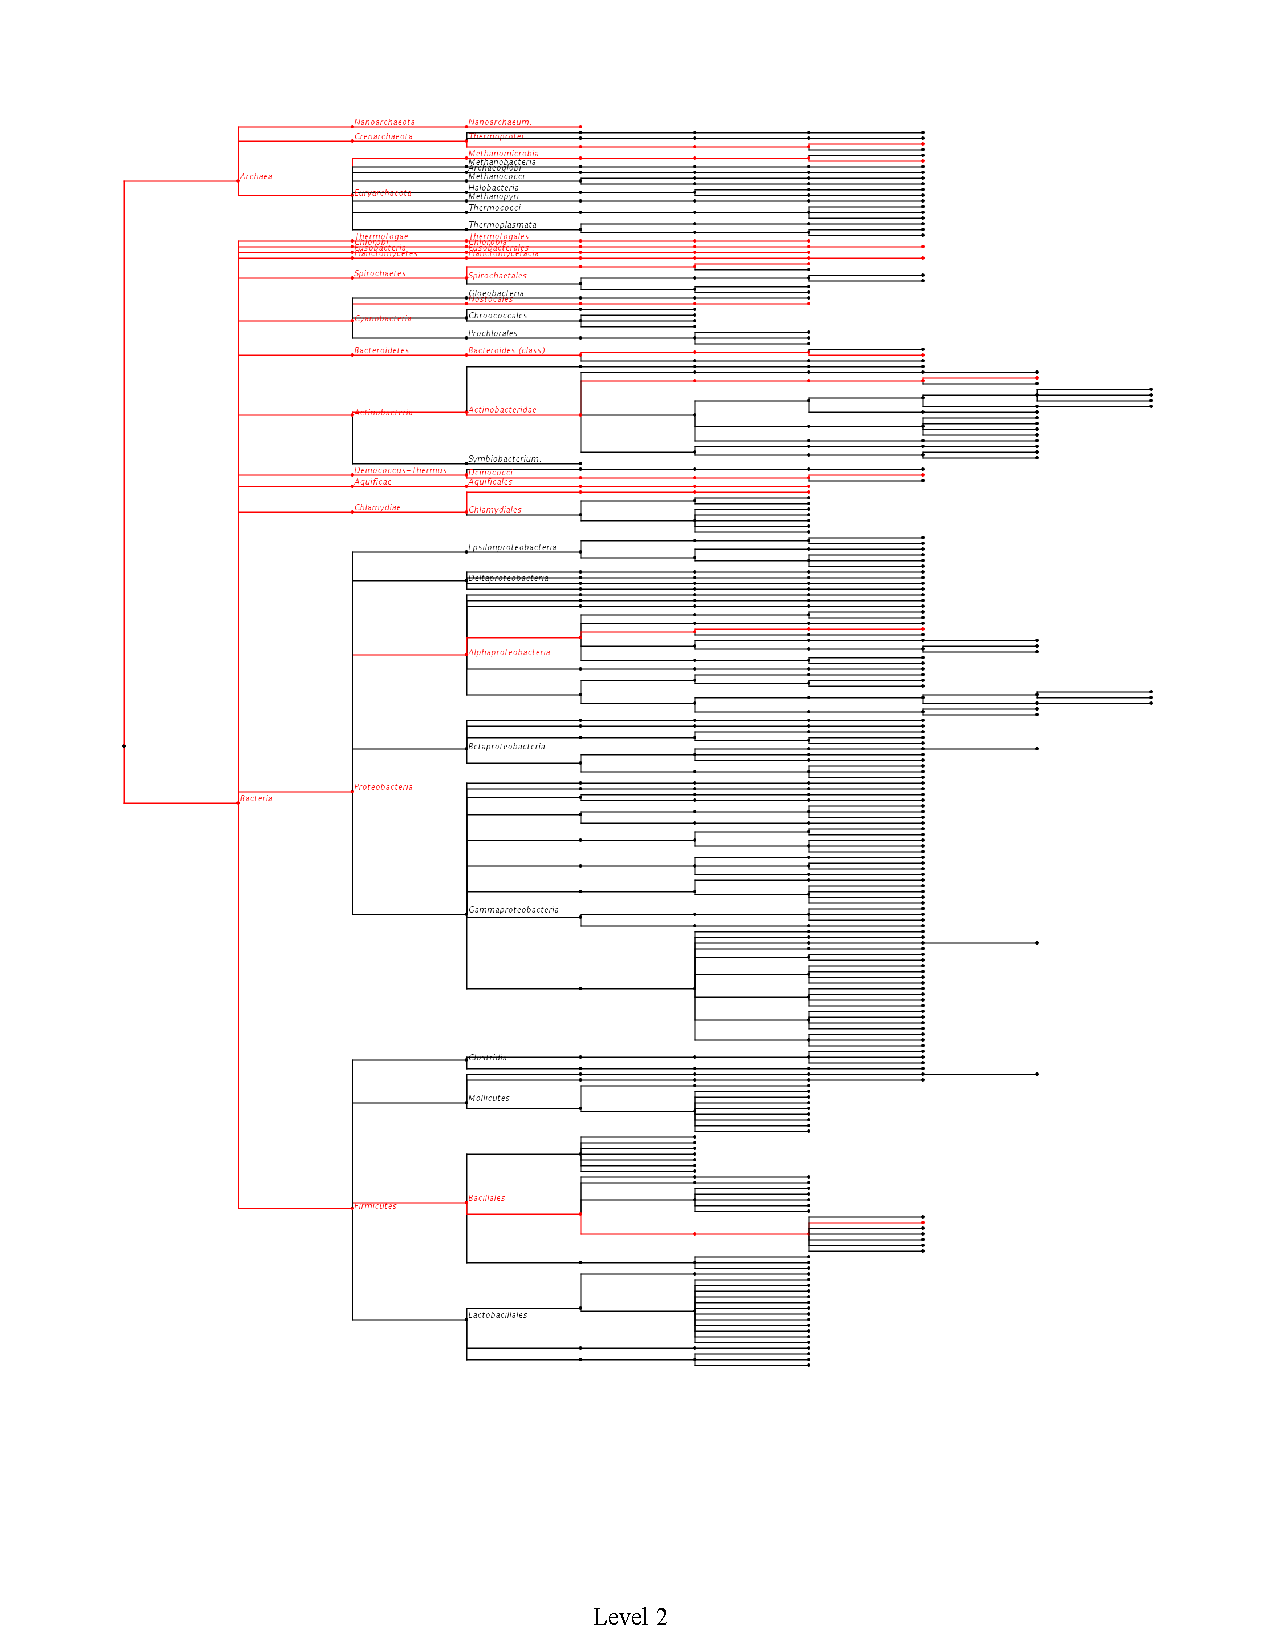
\includepdf[scale=0.9,pages={-},pagecommand={\thispagestyle{fancy}}]{/Users/dochoa/Projects/thesis/thesis.tex/endmatter/dorotaTrees.pdf}

